\documentclass[9pt, aspectratio=169]{beamer}
%\documentclass[9pt, aspectratio=169, handout]{beamer}

\usetheme{metropolis}
\setbeamertemplate{itemize items}{\faAngleRight}

\metroset{titleformat=smallcaps,block=fill,numbering=counter,progressbar=frametitle,sectionpage=none}
\setbeamersize{text margin left=5mm,text margin right=5mm} 
% \input{embed_video}
\usepackage{fontspec}
\usepackage[scale=1]{ccicons}
\usepackage{metalogo}
\usepackage{xcolor,colortbl}
\usepackage{multicol,multirow,booktabs}
\usepackage{appendixnumberbeamer}
\usepackage{graphicx}
\usepackage{svg}
\usepackage{mismath}
\usepackage{bm}
\usepackage{fontawesome5}
\usepackage{csquotes}
%\usepackage[backend=biber, natbib, sorting=nyt, doi=true, url=false, url=false, isbn=false, maxbibnames=10]{biblatex}
%\addbibresource{../../utils/refs.bib}

\usepackage[spanish, es-nodecimaldot]{babel}
\deftranslation[to=spanish]{Definition}{Definición}
\deftranslation[to=spanish]{Theorem}{Teorema}
\deftranslation[to=spanish]{Example}{Ejemplo}

\usepackage{mathtools, mathrsfs}
\usefonttheme{professionalfonts}
\usepackage{textcomp, wasysym}

\setsansfont[BoldFont={Iwona Bold}, Numbers={Lining, Proportional}]{Iwona Light}
% \setmathsfont(Digits)[Numbers={Lining, Proportional}]{Fira Sans Light}
\setmonofont[Scale=MatchLowercase]{DejaVu Sans Mono}

\setbeamercolor{alerted text}{fg=red,bg=black!2}
\setbeamercolor{progress bar}{fg=red,bg=red!2}
\setbeamertemplate{itemize item}{\faCaretRight}
\setbeamertemplate{itemize subitem}{ \faAngleRight}
\setbeamertemplate{blocks}[shadow=false]
\setbeamercolor{block title}{bg=black!30,fg=red}
\setbeamercolor{block body}{bg=black!20,fg=black}
\setbeamertemplate{theorem begin}
{%
\begin{\inserttheoremblockenv}
{%
\inserttheoremheadfont
%{Teorema:}
\inserttheoremname
\ifx\inserttheoremaddition\@empty\else\ : \inserttheoremaddition\fi%
\inserttheorempunctuation
}%
}
\setbeamertemplate{theorem end}{\end{\inserttheoremblockenv}}
\makeatother


 
\usepackage{gensymb,amssymb}
\usepackage{siunitx}
\DeclareSIUnit{\nada}{\relax}
\usepackage{upquote}
\usepackage{cancel}
\usepackage{algpseudocode}
\algrenewcommand\algorithmicrequire{\textbf{Requiere}}
\algrenewcommand\algorithmicensure{\textbf{Devuelve}}
\setbeamertemplate{blocks}[shadow=false]

\newcommand{\cx}{\column{0.5\textwidth}}
\newcommand{\cw}[1]{\column{#1\textwidth}}

\author{Manuel Carlevaro}
\date{}
\institute{
  \vspace{6em}
  \centering
  {\small
  Universidad de Navarra \enspace • \enspace 2024 
} }

%% Operadores
\DeclareMathOperator{\sen}{sen}
\DeclareMathOperator{\senc}{senc}
\DeclareMathOperator{\sign}{sign}
\newcommand{\T}[1]{\underline{\bm{#1}}}
\DeclareMathOperator{\Tr}{Tr}
\DeclareMathOperator{\rg}{rg}
\DeclareMathOperator{\cond}{cond}

\usepackage{hyperref}
\hypersetup{
    colorlinks,
    citecolor=blue,
    filecolor=black,
    linkcolor=blue,
    urlcolor=blue
}
\urlstyle{same}


\usepackage{tikz}
\usetikzlibrary{shapes,shadows,arrows,positioning,matrix,chains,backgrounds,fit}

\tikzset{
    %Define standard arrow tip
    >=stealth',
    %Define style for boxes
    obj/.style={
           rectangle,
           rounded corners,
           draw, very thick,
           text width=10em, fill=green!20,
           minimum height=2em,
           text centered, drop shadow},
    proc/.style={
	    rectangle, rounded corners,
	    draw,fill=red!50,very thick,
	    text width=8em,minimum height=2em,
	    text centered, drop shadow},
    % Define arrow style
    pil/.style={
           ->,
           thick,
           shorten <=2pt,
           shorten >=2pt,}
}

%\setbeamertemplate{bibliography item}{%
  %\ifboolexpr{ test {\ifentrytype{book}} or test {\ifentrytype{mvbook}}
    %or test {\ifentrytype{collection}} or test {\ifentrytype{mvcollection}}
    %or test {\ifentrytype{reference}} or test {\ifentrytype{mvreference}} }
    %{\setbeamertemplate{bibliography item}{\faBook}}
    %{\ifentrytype{online}
            %{\setbeamertemplate{bibliography item}{\faGlobe}}
   %{\setbeamertemplate{bibliography item}{\faFileText}}}%
  %\usebeamertemplate{bibliography item}}

%\defbibenvironment{bibliography}
  %{\list{}
     %{\settowidth{\labelwidth}{\usebeamertemplate{bibliography item}}%
      %\setlength{\leftmargin}{\labelwidth}%
      %\setlength{\labelsep}{\biblabelsep}%
      %\addtolength{\leftmargin}{\labelsep}%
      %\setlength{\itemsep}{\bibitemsep}%
      %\setlength{\parsep}{\bibparsep}}}
  %{\endlist}
  %{\item}
%\newcommand{\bcite}[1]{\citeauthor{#1}, \citetitle{#1} (\citeyear{#1})}


\title{Introducción a las matemáticas}
\subtitle{Conjuntos numéricos}


\begin{document}
\maketitle

\begin{frame}{ Objetivos }
\begin{multicols}{2}
\begin{itemize}
    \item Definir conjuntos por extensión y comprensión. Realizar diagramas de Venn. Identificar elementos y subconjuntos a la vez que relaciones de pertenencia e inclusión.
    \item Realizar operaciones entre conjuntos (unión, intersección y diferencia).
    \item Identificar los conjuntos numéricos.
    \item Revisar la conformación de los números reales: números naturales, enteros, racionales e irracionales.
    \item Conocer la representación del conjunto de los números reales como recta real y los demás conjuntos numéricos.
\item Revisar cómo se manipulan expresiones algebraicas usando las propiedades conmutativas, asociativas y distributivas de las operaciones.
\item Conocer el orden de las prioridades de las operaciones algebraicas y el rol de los paréntesis.
\item Revisar identidades algebraicas importantes que involucran la suma, resta, multiplicación y división.
\end{itemize}
\end{multicols}
\end{frame}

\section{Conjuntos y operaciones entre conjuntos}
\subsection{Definiciones y relaciones de pertenencia e inclusión}

\begin{frame}{Conjuntos y operaciones entre conjuntos}
\begin{definition}[Conjunto]
        Es una colección o agrupamiento de objetos, cosas, etc. Usualmente se utilizan letras mayúsculas para nombrarlos y llaves $\{\}$ para \textbf{escribirlos encerrando sus elementos}.
\end{definition} 
\pause

\begin{example}
\[ S = \{ \text{domingo}, \text{martes}, \text{lunes}, \text{jueves}, \text{viernes}, \text{sábado}, \text{miércoles} \} \]
\end{example} \pause

\textbf{Otros ejemplos:}
\[ A = \{ \text{a}, \text{e}, \text{i}, \text{o}, \text{u} \} \quad B = \{ \text{rojo}, \text{verde}, \text{azul} \} \quad C = \{ \square, \ocircle, \triangle, \diamondsuit, \clubsuit\} \quad  D  = \{1, 2, 3, 4, 5, 6,7 ,8, 9, 0 \}  \]
\pause

\begin{alertblock}{\centering \faInfoCircle}
    \begin{itemize}
        \item \alert{No importa} el orden en que escribimos los elementos de un conjunto.
        \item Tampoco es importante que aparezcan \alert{elementos repetidos}. Por ejemplo, los siguientes conjuntos son iguales:
            \[ \{ \text{a}, \text{b}, \text{c} \} = \{ \text{a}, \text{c}, \text{b}, \text{b}, \text{b} \} = \{ \text{b}, \text{a}, \text{c}, \text{a} \} \]
    \end{itemize}
\end{alertblock}
\end{frame}

\begin{frame}{Conjuntos y operaciones entre conjuntos}
\begin{columns}[t]
\cw{0.45} 
Se utiliza el símbolo ``$\in$'' para indicar que cierto elemento \textbf{pertenece} a un conjunto:
\[ \text{lunes} \in S \]
Se puede leer como ``lunes pertenece a ``$S$''.

Por otro lado, se utiliza el símbolo ``$\notin$'' para indicar que un elemento \textbf{no pertenece} a un conjunto, por ejemplos:
\[ \text{enero} \notin S \]

Cuando el conjunto tiene \textbf{muchos elementos}, o una \textbf{cantidad infinita} de elementos, se utilizan los \textbf{tres puntos} ``$\ldots$'':
\[ \{ \text{a}, \text{b}, \text{c}, \ldots, \text{x}, \text{y}, \text{z} \} \]
\[ \{0, 1, 2, 3, 4, \ldots \} \]
\pause

\cw{0.45}
\textbf{Diagramas de Venn:}
\vspace{1em}

\begin{center}
    
\includegraphics[width=1.0\textwidth]{figs/fig-01.pdf}
\end{center}

\end{columns}
\end{frame}

\begin{frame}{Conjuntos y operaciones entre conjuntos}
\begin{columns}[t]
\cw{0.5}
\begin{definition}[Conjunto vacío]
El conjunto que \textbf{no tiene elementos} se llama ``\textbf{conjunto vacío}'' y se denota con el símbolo ``$\varnothing$'':
\[ \varnothing = \{\} \]
\end{definition}

Con los elementos de un conjunto se pueden formar otros conjuntos ``más pequeños'' que se llaman \textbf{subconjuntos}. Por ejemplo, con $A = \{ \text{a}, \text{e}, \text{i}, \text{o}, \text{u}\}$ se pueden formar varios subconjuntos:
    \begin{align*}
        & \{ \text{e}, \text{i}, \text{o} \} \quad \{ \text{a} \} \quad \{ \text{a}, \text{e} \} \quad \{ \text{i}, \text{u} \}\\
        &\{ \text{i}, \text{o}, \text{u} \} \quad \{ \text{o}, \text{u} \} \quad \{ \text{u}, \text{o}, \text{a}, \text{e} \} \quad \{ \text{o} \}
    \end{align*}
En palabras se dice, por ejemplo, que:
\[ \{ \text{a}, \text{i} \} \txt{es un subconjunto de} \{ \text{a}, \text{e}, \text{i}, \text{o}, \text{u}\} \]

\cw{0.5} o que
\[ \{ \text{a}, \text{i} \} \txt{está incluido en} \{ \text{a}, \text{e}, \text{i}, \text{o}, \text{u}\} \]
\pause

\begin{definition}[$A \subseteq B$]
Se escribe $A \subseteq B$ cuando \textbf{todos los elementos} del conjunto $A$ también son elementos del conjunto $B$. En cambio, se escribe $A \nsubseteq B$ cuando \textbf{algún elemento} de $A$ no es un elemento del conjunto $B$
\end{definition}
\begin{center}
    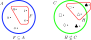
\includegraphics[width=1.0\textwidth]{figs/fig-02.pdf}
\end{center}

\end{columns}
\end{frame}

\begin{frame}{Conjuntos y operaciones entre conjuntos}
    Se puede describir a los conjuntos \textbf{por extensión} o \textbf{por comprensión}. Se dice que un conjunto está descripto por extensión cuando hacemos una lista de sus elementos, como en los ejemplos anteriores:

\[ A = \{ \text{a}, \text{e}, \text{i}, \text{o}, \text{u} \} \quad B = \{ \text{rojo}, \text{verde}, \text{azul} \} \quad C = \{ \square, \ocircle, \triangle, \diamondsuit, \clubsuit\} \quad  D  = \{1, 2, 3, 4, 5, 6,7 ,8, 9, 0 \}  \] 

Por otro lado, se dice que un conjunto está descripto por comprensión cuando se utiliza alguna propiedad característica de sus elementos, por ejemplo:
\[ A = \underbrace{\{ \text{el conjunto de las vocales} \}}_{\text{definición por comprensión}} = \underbrace{ \{ \text{a}, \text{e}, \text{i}, \text{o}, \text{u} \} }_{\text{definición por extensión}} \]

De manera más formal, se utiliza la siguiente notación para definir conjuntos por comprensión:
\[ A = \{ \underbrace{x \text{ es una letra}}_{\text{conjunto con el que trabajamos}} : \underbrace{x \text{ es una vocal}}_{\text{propiedad que debe cumplirse}} \} \]
Se lee: ``$A$ es el conjunto de las letras $x$ \textbf{tal que} $x$ es una vocal''. 
\end{frame}

\begin{frame}{Conjuntos y operaciones entre conjuntos}
\textbf{Ejemplos:}
    \begin{center}
        \begin{tabular}{p{9.5cm} p{4cm}}
            \toprule
            \textbf{Definición por comprensión} & \textbf{Definición por extensión} \\
            \midrule
            $\{ x : x \text{ es una letra de la palabra ``matemática''} \}$ & $\{$m, a, t, e, i , c$\}$ \\
            $\{ x : x \text{ es una vocal de la palabra ``matemática''}\}$ & $\{$a, e, i$\}$ \\
            $\{ x : x \text{ es un Estado miembro de la Unión Europea que empieza con ``F''}\}$ & $\{$Francia, Finlandia$\}$ \\
            $\{ x : x \text{ es un dígito decimal par}\}$ & $\{0, 2, 4, 6, 8\}$ \\
            \bottomrule
        \end{tabular}
    \end{center}

\vspace{3em}
\begin{center}
    {\Large \alert{\faArrowCircleRight \faPen* Actividad 1}}
\end{center}
\end{frame}

\subsection{Operaciones entre conjuntos}

\begin{frame}{Operaciones entre conjuntos: intersección}
\begin{columns}[c]
\cx
\begin{definition}[Intersección de conjuntos]
    La \textbf{intersección} de dos conjuntos es un nuevo conjunto formado por los elementos que están en ambos conjuntos simultáneamente. Considerando $A$ y $B$ dos conjuntos, escribimos la intersección de $A$ y $B$ de la siguiente forma:
    \[ A \cap B = \{ x : x \in A \text{ y } x \in B \} \]
\end{definition}

\begin{example}
    Si $A = \{$a, b, c, g$\}$ y $B = \{$r, g$\}$, entonces:
    \[ A \cap B = \{\text{g} \} \]
\end{example}

\cx
\begin{center}
    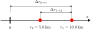
\includegraphics[scale=1.0]{figs/fig-03.pdf}
\end{center}
\end{columns}
\end{frame}

\begin{frame}{Operaciones entre conjuntos: unión}
\begin{columns}[c]
\cx
\begin{definition}[Unión de conjuntos]
    La \textbf{unión} de dos conjuntos es un nuevo conjunto formado por los elementos que están en uno u otro conjunto. Considerando $A$ y $B$ dos conjuntos, escribimos la unión de $A$ y $B$ de la siguiente forma:
    \[ A \cup B = \{ x : x \in A \text{ o } x \in B \} \]
\end{definition}

\begin{example}
    Si $A = \{$a, b, c, g$\}$ y $B = \{$r, g$\}$, entonces:
    \[ A \cup B = \{\text{a}, \text{b}, \text{c}, \text{r}, \text{g} \} \]
\end{example}

\cx
\begin{center}
    
\includegraphics[scale=1.0]{figs/fig-04.pdf}
\end{center}
\end{columns}
\end{frame}

\begin{frame}{Operaciones entre conjuntos: diferencia}
\begin{columns}[c]
\cx
\begin{definition}[Diferencia de conjuntos]
    La \textbf{diferencia} del conjunto $A$ con el conjunto $B$ es un nuevo conjunto formado por todos los elementos de $A$ que no están en $B$. Considerando $A$ y $B$ dos conjuntos, escribimos la diferencia de $A$ con $B$ de la siguiente forma:
    \[ A - B = \{ x : x \in A \text{ y } x \notin B \} \]
\end{definition}

\begin{example}
    Si $A = \{$a, b, c, g$\}$ y $B = \{$r, g$\}$, entonces:
    \[ A - B = \{\text{a}, \text{b}, \text{c} \} \]
\end{example}

\cx
\begin{center}
    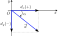
\includegraphics[scale=1.0]{figs/fig-05.pdf}
\end{center}
\end{columns}
\end{frame}

\begin{frame}{Operaciones entre conjuntos}
\begin{block}{Ejemplo:}
23 estudiantes de un curso practican alguno de los siguientes deportes: tenis, fútbol y voley. Cuatro de ellas juegan regularmente los tres deportes; cinco juegan solamente voley y fútbol; dos juegan solamente tenis y fútbol; y tres juegan solamente tenis y voley. Además, tres personas juegan únicamente tenis y una persona juega únicamente fútbol. ¿Cuantas personas juegan únicamente voley?
\vspace{-2.5em}
\begin{center}
\[ T = \{\text{estudiantes que juegan tenis}\}; V = \{\text{estudiantes que juegan voley}\}; F = \{\text{estudiantes que juegan fútbol}\} \]
\end{center}
\end{block} \pause
\begin{columns}[c]
\cw{0.6}
{\small
\begin{tabular}{ccc}
\toprule
\textbf{Enunciado} & \textbf{Conjunto} & \textbf{\# elementos} \\
\midrule
Total de alumnos & $V \cup F \cup T$ & 23 \\
Alumnos que juegan 3 deportes & $V \cap F \cap T$ & 4 \\
Alumnos que juegan únicamente voley y fútbol& $(V \cap F) - T$ & 5 \\
Alumnos que juegan únicamente tenis y fútbol& $(T \cap F) - V$ & 2 \\
Alumnos que juegan únicamente tenis y voley& $(T \cap V) - F$ & 3 \\
Alumnos que juegan únicamente tenis& $T - (V \cup F) $ & 3 \\
Alumnos que juegan únicamente fútbol& $F - (T \cup V) $ & 1 \\
Alumnos que juegan únicamente voley& $V - (T \cup F) $ & ¿? \\
\bottomrule
\end{tabular}
}
\cw{0.4}
\begin{center}
    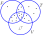
\includegraphics[scale=1.0]{figs/fig-06.pdf}
\end{center}
\end{columns}
\pause

\begin{center}
    {\Large \alert{\faArrowCircleRight \faPen* Actividad 2}}
\end{center}
\end{frame}

\section{Conjuntos numéricos}

\begin{frame}{Conjuntos numéricos}
\begin{columns}[t]
\cx
\begin{definition}[Números naturales]
    Utilizamos los \textbf{números naturales} para contar cosas. Denotamos este conjunto con el símbolo $\mathbb{N}$:
\[ \mathbb{N} = \{0, 1, 2, 3, 4, \ldots \} \]
Consideramos al $0$ como número natural, aunque algunos libros no lo hacen.
\end{definition}
\cx
\begin{definition}[Números enteros]
    Los \textbf{números enteros} están comprendidos por los naturales y sus opuestos. Utilizamos el símbolo $\mathbb{Z}$ para este conjuntos:
\[ \mathbb{Z} = \{\ldots, -4, -3, -2, -1, 0, 1, 2, 3, 4, \ldots \} \]
\end{definition}
\end{columns}

\textbf{Representación gráfica:}
\begin{center}
    
\includegraphics[width=0.75\textwidth]{figs/fig-12.pdf}
\end{center}
\end{frame}

\begin{frame}{Conjuntos numéricos}
    \begin{columns}[c]
\cx
\begin{definition}[Números racionales o fraccionarios]
    Son aquellos números que pueden escribirse como \textbf{cociente} entre dos números enteros:
    \[ \frac{p}{q} = \frac{\text{numerador}}{\text{denominador}} = \frac{\text{número entero}}{\text{número entero } \neq 0} \]
    Utilizamos el símbolo $\mathbb{Q}$ para denotar este conjunto: 
    \[ \mathbb{Q} = \{ 0, 1, -3, \frac{1}{3}, \frac{5}{2}, \ldots, -4, 0.3, \ldots, \} \]
\end{definition}
\cx
\begin{center}
    \includesvg[scale=1.0]{figs/fig-13.svg}
\end{center}
\end{columns}
\end{frame}

\begin{frame}{Conjuntos numéricos}
    Los números fraccionarios también tienen su representación en \textbf{forma decimal}. En este caso podemos obtener decimales exactos o decimales periódicos (que se van repitiendo indefinidamente):
    \[ \frac{1}{2} = \underbrace{0.5}_{\text{decimales exactos}} \qquad \frac{2}{3} = \underbrace{0.\hat{6} = 0.66666\ldots}_{\text{decimales periódicos}} \]
\pause

\textbf{Representación gráfica:} En la representación lineal, en cualquier segmento (sin importar su tamaño) se pueden encontrar números fraccionarios. Entre dos números fraccionarios existen una infinidad de otros números racionales:
\begin{columns}[c]
\cw{0.7}
\begin{center}
    \includegraphics[width=0.90\textwidth]{figs/racionales.png}
\end{center}
\pause
\cw{0.3}
¿Se puede completar toda la línea numérica con números racionales? La respuesta es \textbf{negativa}, y se debe a que algunas longitudes o magnitudes no son números racionales, sino \textbf{irracionales}.
\end{columns}
\end{frame}

\begin{frame}
\begin{columns}[t]
\cx
\begin{definition}[Números irracionales]
    Son aquellos números que \textbf{no pueden escribirse} como cociente de dos números enteros. Usamos el símbolo $\mathbb{I}$ para denotar a este conjunto:
    \[ \mathbb{I} = \{ \sqrt{2}, -\sqrt[3]{5}, \pi, e, \ldots \} \]
\end{definition}

Al escribir los números racionales en \textbf{forma decimal} siempre obtenemos una expresión con infinitas cifras no periódicas:
\[ \pi = \underbrace{3.141592654\ldots}_{\text{decimales no periódicos}} \quad \sqrt{2} = \underbrace{1.414213562\ldots}_{\text{decimales no periódicos}} \]
\pause

\cx
\begin{definition}[Números reales]
    Es la unión de los números racionales y los irracionales, conformando la totalidad de los \textbf{números reales} que permiten calcular cualquier longitud posible. Utilizamos el símbolo $\mathbb{R}$ para llamar a este conjunto:
\[ \mathbb{R} = \{0, -1, \frac{1}{3}, \sqrt{2}, -\sqrt{5}, \pi, \frac{7}{3}, \ldots \} \]
\end{definition}
\begin{center}
    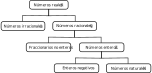
\includegraphics[scale=0.5]{figs/fig-14.pdf}
\end{center}
\end{columns}
\end{frame}

\begin{frame}{Otros conjuntos numéricos}
\begin{columns}[t]
\cx
\begin{definition}[Números pares]
    Son los \textbf{números enteros divisibles por 2}. En forma simbólica:
    \[ n = 2 \, p, \quad p \in \mathbb{Z} \]
\end{definition}
Cualquier entero que termine en 0, 2, 4, 6 u 8 es un número par:
\[ \{\ldots, -1240, -238, -156, -2, 0, 2, 4, 16, 88, 12340, \ldots \} \]
\[ \{ n \in \mathbb{Z} : n = 2 \, p \txt{para algún} p \in \mathbb{Z} \} \]
\pause

\cx
\begin{definition}[Números impares]
    Son los \textbf{números enteros que no divisibles por 2}. En forma simbólica:
    \[ n = 2 \, p + 1, \quad p \in \mathbb{Z} \]
\end{definition}
Cualquier entero que termine en 1, 3, 5, 7 u 9 es un número impar:
\[ \{\ldots, -12345, 99, -1, 1, 3 17, 23,\ldots \} \]
\[ \{ n \in \mathbb{Z} : n = 2 \, p + 1 \txt{para algún} p \in \mathbb{Z} \} \]
\end{columns}
\end{frame}

\begin{frame}{Otros conjuntos numéricos}
\begin{columns}[t]
\cx
\begin{definition}[Números primos]
    Son los \textbf{números naturales mayores que 1 divisibles solo por sí mismos y la unidad}.
\end{definition}
Los primeros 5 números primos son 2, 3, 5, 7, y 11.

Los números primos pueden ser muy útiles para factorizar números enteros y facilitar las operaciones entre fracciones.
\pause

\cx
\begin{definition}[Números compuestos]
    Son los \textbf{números naturales mayores que 1 que tienen algún divisor natural aparte de sí mismos y el 1}. 
\end{definition}

Los primeros 5 números compuestos son 4, 6, 8, 9, 10.
\end{columns}
\vfill
\begin{center}
    {\Large \alert{\faArrowCircleRight \faPen* Actividad 3}}
\end{center}
\end{frame}

\section*{Operaciones algebraicas}

\begin{frame}{Operaciones algebraicas}
    Propiedades de la \textbf{suma} y de la \textbf{multiplicación}: $a$, $b$ y $c$ son números reales.

\begin{center}
    \begin{tabular}{ccc}
    \toprule
    & \textbf{Suma} & \textbf{Multiplicación} \\
    \midrule
        Propiedad de cierre & $a + b \in \mathbb{R}$ & $a \mul b \in \mathbb{R}$ \\
        Propiedad conmutativa & $a + b = b + a$ & $a \mul b = b \mul a$ \\
        Propiedad asociativa & $(a + b) + c = a + (b + c)$ & $(a \mul b) \mul c = a \mul (b \mul c)$ \\
        Elemento neutro & $a + 0 = a$ & $a \mul 1 = a$ \\
        Números opuestos/inversos & $a + (-a) = 0$ & $a \mul a^{-1} = 1, a \neq 0$ \\
        Propiedad distributiva & \multicolumn{2}{c} {$a \mul (b + c) = a \mul b + a \mul c$} \\
    \bottomrule
    \end{tabular}
\end{center}
\end{frame}

\begin{frame}{Operaciones algebraicas}
\begin{block}{Notación para el producto}
    La forma más usual es usando un \textbf{punto en el medio del renglón}, pero también se usa el símbolo $\mul$ y paréntesis:
    \[ 15 = \underbracket{3 \mul 5}_{\text{usando }\mul} = \overbracket{3 \cdot 5}^{\text{usando } \cdot} = \underbracket{(3)(5) = 3(5) = (3)5}_{\text{usando }()} \]
Cuando se utilizan letras o variables está permitido no usar símbolos o paréntesis entre medio:
\[ 3 a = 3 \cdot a \qquad ab = a \cdot b \]
Sin embargo, \textbf{se evita} usar la escritura anterior cuando se trata de números propiamente dichos para evitar confusión:
\[ 35 = \text{treinta y cinco} \qquad 35 \stackrel{\textcolor{red}{\text{NO ES}}}= 3 \cdot 5 \]
\end{block}
\end{frame}

\begin{frame}{Operaciones algebraicas}
    \begin{block}{Cambio de precedencia en las operaciones aritméticas}
        La \textbf{regla principal} cuando usamos \textbf{paréntesis} y/o \textbf{corchetes} es que debe respetarse el orden de las operaciones indicadas siempre desde los más internos y luego avanzando hacia \textbf{afuera}:
        \[ 3[\underbracket{(3+4)}_{\text{\usym{2780}}} - \underbracket{(2+2)}_{\text{\usym{2780}}}] = 3 \overbracket{[7 -  4] }^{\text{\usym{2781}}} = \underbracket{3 \cdot 3}_{\text{\usym{2782}}} = 9 \]
    \end{block}
\end{frame}

\begin{frame}{Operaciones algebraicas}
    \begin{block}{Resta y división}
        \vspace{0.3em}
        \begin{columns}
            \cw{0.45}
            \textbf{Resta:} para $a, b \in \mathbb{R}$
            \[ a - b = a + (-b) \]
            \cw{0.45}
            \textbf{División:} para $a, b \in \mathbb{R}, b \neq 0$
            \[ a \div b = a \mul \frac{1}{b} \]
        \end{columns}
    \end{block}

    \begin{block}{Notación}
Para la división se utilizan varios símbolos o notaciones:
\[ a \div b \qquad a : b \qquad a/b \qquad \frac{a}{b} \]
Los símbolos de las operaciones \textbf{nunca se escriben juntos}, se deben usar paréntesis o corchetes:
\begin{columns}[t]
    \cw{0.45}
    \begin{center}
        Formas correctas
    \end{center}
    \[ 3 +(-2) \quad 3 \cdot(-12) \quad -9 \div(-2) \]
    \cw{0.45}
    \begin{center}
        Formas incorrectas
    \end{center}
    \[ 3 + -2 \quad 3 \cdot -12  \quad -9 \div -2 \]
\end{columns}
    \end{block}
\end{frame}

\begin{frame}{Operaciones algebraicas}
    \textbf{Propiedades de la resta (o de los números opuestos):}
    \begin{itemize}
        \item Calcular el opuesto es lo mismo que multiplicar por $-1$: $-a = (-1) \cdot a$
        \item El \textbf{doble} opuesto: $-(-a) = (-1) \cdot (-1) \cdot a = a$
        \item Números opuestos y multiplicación: $-a \cdot b = -(a \cdot b) = (-a) \cdot b = a \cdot (-b)$
        \item Números opuestos y fracciones: para $b \neq 0$, 
            \[ -\frac{a}{b} = \frac{-a}{b} = \frac{a}{-b} \txt{y} \frac{-a}{-b} = \frac{a}{b} \]
        \item \textbf{Distributiva} de negativo: $-(a + b) = -a - b \txt{y} -(a - b) = -a + b$
    \end{itemize}
\end{frame}

\begin{frame}{Operaciones algebraicas}
    \textbf{Propiedades de la división (o de los números inversos):} $a, b, c$ y $d$ son números reales aclarando que cuando corresponda el numerador es diferente de cero.
\begin{itemize}
\item \textbf{Suma} de fracciones con \textbf{igual denominador}: es la forma más simple de sumar fracciones porque se considera que se están sumando cantidades de una misma fracción de la unidad (se suman directamente los numeradores):
    \[ \frac{a}{b} + \frac{c}{b} = a \cdot \frac{1}{b} + c \cdot \frac{1}{b} = (a + c) \cdot \frac{1}{b} = \frac{a + c}{b} \]
\item \textbf{Suma} de fracciones en general: se buscan \textbf{fracciones equivalentes} que tengan el mismo denominador:
    \[ \frac{a}{b} + \frac{c}{d} \stackrel{\text{\textcolor{red}{equivalentes}}}{=} \frac{ad}{bd} + \frac{cb}{db} \stackrel{\text{\textcolor{red}{igual denominador}}}{=} \frac{ad + cb}{bd} \]
\item \textbf{Multiplicación} de fracciones: se calculan multiplicando numeradores entre sí y denominadores entre sí:
    \[ \frac{a}{b} \cdot \frac{c}{d} = \frac{ac}{bd} \]
\item \textbf{División} de fracciones: la segunda función \textbf{se da vuelta} y luego se multiplica: 
    \[ \frac{a}{b} \div \frac{c}{d} = \frac{a}{b} \cdot \frac{d}{c} = \frac{ad}{bc} \]
\end{itemize}
\end{frame}

\begin{frame}{Operaciones algebraicas}
    \textbf{Suma de fracciones usando mínimo común múltiplo:} ejemplos:
\begin{itemize}
    \item $1/6 + 2/3 + 4/9$. Los denominadores son 6, 3 y 9 cuyo mínimo común múltiplo es 18. Las fracciones equivalentes son:
        \[ \frac{1}{6} = \frac{1}{6} \cdot \frac{3}{3} = \frac{3}{18} \qquad \frac{2}{3} = \frac{2}{3} \cdot \frac{6}{6} = \frac{12}{18} \qquad \frac{4}{9} = \frac{4}{9} \cdot \frac{2}{2} = \frac{8}{18} \]
        Entonces:
        \[ \frac{1}{6} + \frac{2}{3} + \frac{4}{9} = \frac{3}{18} + \frac{12}{18} + \frac{8}{18} = \frac{3 +12 + 8}{18} = \frac{23}{18} \]
\item $2 + 5/8 - 5/6$. Los denominadores son 1, 8  y 6, con mínimo común múltiplo 24:
    \[ 2 + \frac{5}{8} - \frac{5}{6} = \frac{48}{24} + \frac{15}{24} - \frac{20}{24} = \frac{48 + 15 - 20}{24} = \frac{43}{24} \]
\end{itemize}
\end{frame}

\begin{frame}{Operaciones algebraicas}
    \begin{definition}[Potenciación]
        \begin{itemize}
            \item Exponente $n \in \mathbb{N} - \{0\}$:
                \[ a^n = \underbrace{a \cdot a \cdot a \cdot \ldots \cdot a}_{n \text{ veces}} \]
            \item Caso particular $n = 0$, $a \neq 0$: $a^0 = 1$
            \item $n = 0$ y $a = 0$ \alert{no está definida matemáticamente}: $0^0$ expresión \textbf{no definida}.
            \item Para $a \neq 0$ se calculan potencias con números enteros \textbf{negativos}:
                \[ a^{-n} = \frac{1}{a^n} \]
        \end{itemize}
    \end{definition}

\end{frame}

\begin{frame}{Operaciones algebraicas}
    \textbf{Ejemplos:}
\begin{multicols}{2}
\begin{itemize}
\item $5^3 = 5 \cdot 5 \cdot 5 = 125$
\item $(-2)^4 = (-2) \cdot (-2) \cdot (-2) \cdot (-2) = 16$
\item \[\pow{\frac{3}{7}}{2} = \left(\frac{3}{7}\right) \cdot \left(\frac{3}{7}\right) = \frac{9}{49} \]
\item $x^3 = x \cdot x \cdot x$
\item $a^1 = a$
\item \[ \pow{\frac{234}{1354}}{0} = 1 \]
\item \[ 2^{-3} = \frac{1}{2^3} = \frac{1}{8} \]
\item \[ (-3)^{-2} = \frac{1}{(-3)^2} = \frac{1}{9} \] 
\end{itemize}
\end{multicols}
\end{frame}

\begin{frame}{Operaciones algebraicas}
    \textbf{Propiedades de las potencias con exponentes enteros}: $a$ y $b$ son números reales diferentes de cero, $n, m \in \mathbb{Z}$:
\begin{itemize}
    \item \textbf{Regla del producto}: producto de potencias de \textbf{igual base}, se \textbf{suman} los exponentes: $a^n \cdot a^m = a^{n+m}$:
        \[ a^n \cdot a^m = \underbrace{a \cdot \ldots \cdot a}_{n \text{ veces}} \cdot \underbrace{a \cdot \ldots \cdot a}_{m \text{ veces}} = a^{n+m} \]
    \item \textbf{Distributiva respecto de la multiplicación:} $(a \cdot b)^n = a^n \cdot b^n$:
        \[ (a \cdot b)^n = \underbrace{(a \cdot b) \cdot \ldots \cdot (a \cdot b)}_{n \text{ veces}} = \underbrace{a \cdot \ldots \cdot a}_{n \text{ veces}} \cdot \underbrace{b \cdot \ldots \cdot b}_{n \text{ veces}} = a^n \cdot b^n \]
    \item \textbf{Regla del cociente:} en una división de potencias de \textbf{igual base} se \textbf{restan} los exponentes: $a^n/a^m = a^{n-m}$. Para el caso de $n > m$:
        \[ \frac{a^n}{a^m} = \frac{\overbrace{a \cdot \ldots \cdot a}^{n \text{ veces}}}{\underbrace{a \cdot \ldots \cdot a}_{m \text{ veces}}} = \underbrace{a \cdot \ldots \cdot a}_{n - m \text{ veces}} = a^{n-m}\]
\end{itemize}
\end{frame}


\begin{frame}{Operaciones algebraicas}
    \textbf{Propiedades de las potencias con exponentes enteros}: (continuación)
\begin{itemize}
    \item \textbf{Distributiva respecto de la división:} $(a/b)^n = a^n / b^n$:
        \[ \left(\frac{a}{b}\right)^n = \underbrace{\left(\frac{a}{b}\right) \cdot \ldots \cdot \left(\frac{a}{b}\right)}_{n \text{ veces}}  = \frac{\overbrace{a \cdot \ldots \cdot a}^{n \text{ veces}}}{\underbrace{a \cdot \ldots \cdot a}_{n \text{ veces}}} = \frac{a^n}{b^n} \]
    \item \textbf{Regla de la potencia:} en una potencia dentro de otra potencia, los exponentes se \textbf{multiplican}: $(a^n)^m = a^{n\cdot m}$
        \[ (a^n)^m = \underbrace{\underbrace{(a \cdot \ldots \cdots a)}_{n \text{ veces}} \cdot \ldots \cdot \underbrace{(a \cdot \ldots \cdots a)}_{n \text{ veces}}}_{m \text{ veces}} = \underbrace{a \cdot \ldots \cdot a}_{m \cdot n \text{ veces}} = a^{n \cdot m} \]
    \item \textbf{Regla de la potencia opuesta:} Si la potencia es negativa, la fracción se invierte y se cambia de signo el exponente: 
        \[ \left(\frac{a}{b}\right)^{-n} = \left(\frac{b}{a}\right)^n \qquad \text{\textcolor{red}{¡Cuidado! }} (-3)^2 = (-3)\cdot(-3) = 9 \neq -3^2 = -(3^2) =  -3 \cdot 3 = -9 \]
\end{itemize}
\end{frame}

\begin{frame}{Operaciones algebraicas}
\begin{columns}[c]
\cx 
\begin{definition}[Radicación]
Es el proceso de hallar las raíces de orden $n$ de un número $a$. Para números reales:
\[ \sqrt[n]{a} = x \]
donde:
\begin{itemize}
    \item $n$ es el \textbf{índice} u \textbf{orden}, $a$ es el \textbf{radicando}.
    \item Según $n$ sea impar o par:
        \begin{itemize}
            \item $n$ impar $\mapsto \sqrt[n]{a} = x$ \textbf{raíz enésima}.
            \item $n$ par $\mapsto \sqrt[n]{a} = \pm x$ \textbf{raíces enésimas}.
        \end{itemize}
    \item Si $a < 0$ solo existe la raíz real si $n$ es impar.
\end{itemize}
\end{definition}
\pause
\begin{alertblock}{\centering \faExclamationTriangle}
    La raíz cuadrada de los números enteros, si estos no son cuadrados perfectos, son siempre números irracionales.
\end{alertblock}
\pause
\cx 
\textbf{Propiedades:}
\begin{multicols}{2}
    \begin{itemize}
    \item $ \sqrt[np]{a^p} = \sqrt[n]{a} $
    \item $ \sqrt[n]{a \cdot b} = \sqrt[n]{a} \cdot \sqrt[n]{b} $
    \item $\sqrt[n]{\frac{a}{b}} = \frac{\sqrt[n]{a}}{\sqrt[n]{b}}$
    \item $\left(\sqrt[n]{a}\right)^p = \sqrt[n]{a^p}$
    \item $\sqrt[m]{\sqrt[n]{a}} = \sqrt[m \cdot n]{a}$
    \item $\sqrt[m]{a} \cdot \sqrt[n]{a} = \sqrt[m \cdot n]{a^{m + n}}$
\end{itemize}
\end{multicols}
\textbf{Nota:} la raíz enésima de un número se puede poner en forma de potencia:
\[ \sqrt[n]{a} = a^{1/n} \] 
ya que
\[ (\sqrt[n]{a})^n = a \txt{y} (a^{1/n})^n = a^{n/n} = a \]

\vfill
\begin{center}
    {\Large \alert{\faArrowCircleRight \faPen* Actividad 4}}
\end{center}
\end{columns}
\end{frame}
\end{document}

